\documentclass{beamer}
\usepackage{hyperref}

\title{Generative Adversarial Networks}
\author{Santhisenan A}
\institute{Department of Computer Science \& Engineering
\\ College of Engineering Trivandrum}
\date{\today}


\begin{document}

\frame{\titlepage}

\begin{frame}
\frametitle{Overview}
\tableofcontents
\end{frame}

\begin{frame}{GAN}
    \begin{itemize}
        \item{\textbf{G}enerative}
            \begin{itemize}
                \item {}
            \end{itemize}
        \item{\textbf{A}dversarial}
        \item{\textbf{N}etwork}
    \end{itemize}
\end{frame}  

\begin{frame}
    \frametitle{Supervised vs Unsupervised learning}
    \begin{columns}
        \column{0.5\textwidth}
            {\Large Supervised learning} \\
            \textbf{Data}:
            \begin{itemize}
                \item{x, the input data}
                \item{y, the output label}
            \end{itemize}
            \textbf{Goal} $-$ learn a function that to map from x to y \\
            \textbf{Examples} $-$ Classification, regression, object detection, etc.
            
            \column{0.5\textwidth}

    \end{columns}

\end{frame}

\begin{frame}
    \frametitle{Supervised vs Unsupervised learning}
    \begin{columns}
        \column{0.5\textwidth}
            {\Large Supervised learning} \\
            \textbf{Data}:
            \begin{itemize}
                \item{x, the input data}
                \item{y, the output label}
            \end{itemize}
            \textbf{Goal} $-$ learn a function that to map from x to y \\
            \textbf{Examples} $-$ Classification, regression, object detection, etc.
        
        \column{0.5\textwidth}
            {\Large Unsupervised learning} \\
            \textbf{Data}:
            \begin{itemize}
                \item{x, the input data}
                \item{No labels}
            \end{itemize}
            \textbf{Goal} $-$ learn some underlying hidden structure of data\\
            \textbf{Examples} $-$  Clustering, dimensionality reduction, etc.
    \end{columns}
\end{frame}

\begin{frame}
    \frametitle{Supervised vs Unsupervised learning}
    \begin{columns}
        \column{0.5\textwidth}
            {\Large Supervised learning} \\
            \textbf{Data}:
            \begin{itemize}
                \item{x, the input data}
                \item{y, the output label}
            \end{itemize}
            \textbf{Goal} $-$ learn a function that to map from x to y \\
            \textbf{Examples} $-$ Classification, regression, object detection, etc.
        
        \column{0.5\textwidth}
            {\Large Unsupervised learning} \\
            \textbf{Data}:
            \begin{itemize}
                \item{x, the input data [{\small \color{blue} the training data is cheap}]}
                \item{No labels}
            \end{itemize}
            \textbf{Goal} $-$ learn some underlying hidden structure of data \\
            \textbf{Examples} $-$  Clustering, dimensionality reduction, etc.
    \end{columns}
\end{frame}

\begin{frame}
    \frametitle{Generative Models}
    \begin{itemize}
        \item Given a training set, generate new samples that are similar to the 
        data in the training set.
    \end{itemize}
        \begin{columns}
            \column{0.5\textwidth}
            \begin{center}
                \begin{figure}
                    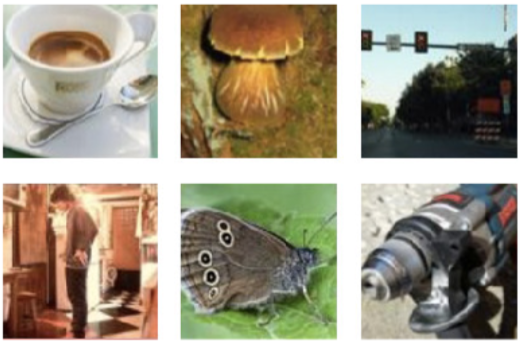
\includegraphics[width=0.5\textwidth]{images/trainset.png}
                \end{figure}
                {Training data $p _{data} (x)$}
            \end{center}
            
            \column{0.5\textwidth}
            \begin{center}
                \begin{figure}
                    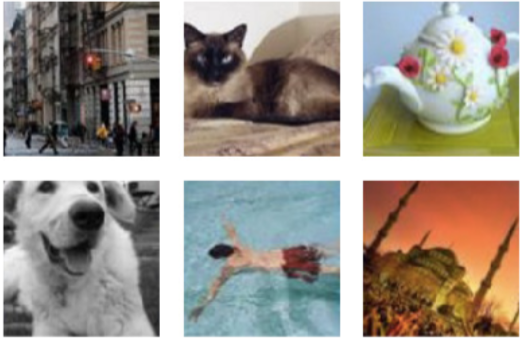
\includegraphics[width=0.5\textwidth]{images/modeloutput.png}
                \end{figure}
                {Generated samples $p _{model} (x)$} \\
            \end{center}
        \end{columns}
        \footnote{[Source: NIPS 2016 tutorial on GANs by \textit{Ian Goodfellow}]}
        \begin{center}
            \pause\color{blue}\Large{We want  $p _{model} (x)$ to be similar to $p _{data} (x)$}
        \end{center}
\end{frame}

\begin{frame}
    \frametitle{Adversarial training}
    \begin{itemize}
        \item {The term has been used by computer scientists for a long time.}
        \item {Current usage: "Training a model in the worst case scenario, with inputs chosen 
        by an adverasary."}
        \item {Examples:
        \begin{itemize}
            \item  {An agent playing against a copy of itself in a board game 
            (Samuel's Checkers-playing Program, 1959)}
            \item  {Generative adversarial Networks (Ian Goodfellow \textit{et. al}, 2014)}
        \end{itemize}}
    \end{itemize}
\end{frame}

\begin{frame}
    \frametitle{Generative Adversarial Networks}
    GANs \footnote{Ian Goodfellow et al., “Generative Adversarial Nets”, NIPS 2014} 
    consists of two neural networks $-$
    \begin{itemize}
        \item \textbf{Generator (G)} which tries of generate new data.
        \pause \item \textbf{Discriminator (D)} which tries to classify the data 
        given as input to it as "real" or "fake".
    \end{itemize}
\end{frame}

\begin{frame}{The framework}
    \begin{center}
        \begin{figure}
            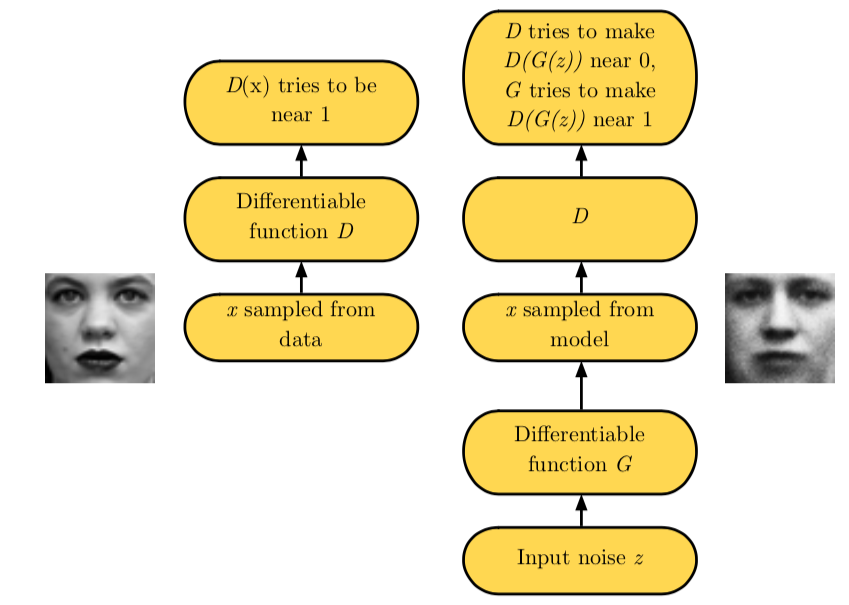
\includegraphics[width=0.9\textwidth]{images/advernetfmk.png}
        \end{figure}
    \end{center}
    \footnote{Ian Goodfellow, NIPS 2016 tutorial on GANs}
\end{frame}

\begin{frame}
    \frametitle{An analogy - Counterfeiters and Police}
    \begin{itemize}
        \item {Police should allow people with real money to safely spend their money.}
        \pause \item {Police should also catch counterfeit money and remove it from circulation and punish the counterfeiters.}
        \pause \item {The counterfeiters will try to fool the police and use their money.}
        \pause \item {Over time, the police learn to be better at catching fake currency and 
        the counterfeiters learn to be better at producing fake currency.}
        \pause \item {The equilibrium is reached when the counterfeiters learn to produce fake 
        currency which cannot be distinguished from the real currency.}
    \end{itemize}
\end{frame}

\begin{frame}
    \frametitle{Image to Image translation \footnote{Image-to-Image Translation 
    with Conditional Adversarial Networks, Isola et. al 2016}}
    \begin{columns}
        \column{0.5\textwidth}
            \begin{center}
                \begin{figure}
                    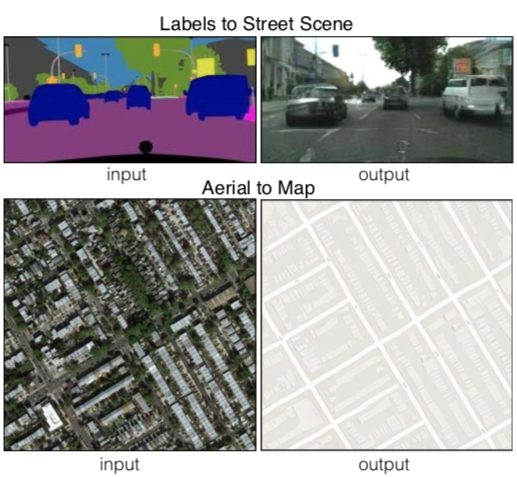
\includegraphics[width=0.9\textwidth]{images/img2img2.png}
                \end{figure}
            \end{center}
        \column{0.5\textwidth}
            \begin{center}
                \begin{figure}
                    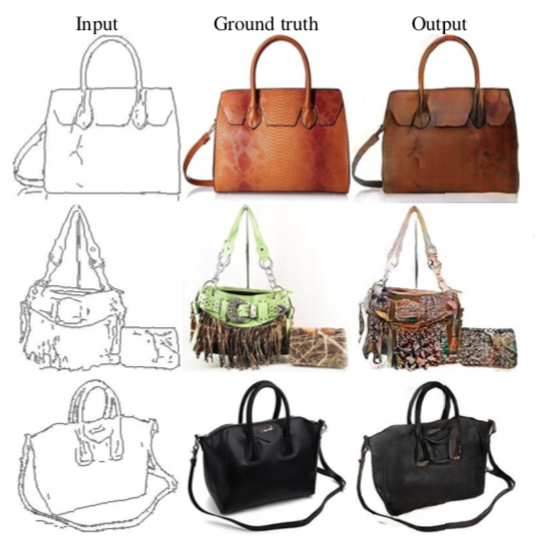
\includegraphics[width=0.9\textwidth]{images/img1img1.png}
                \end{figure}
            \end{center}            
    \end{columns}
\end{frame}

\begin{frame}
    \frametitle{Generative Adversarial Text to Image Synthesis 
    \footnote{Generative Adversarial Text to Image Synthesis, Scott Reed et. al, ICML 2016}}
    \begin{center}
        \begin{figure}
            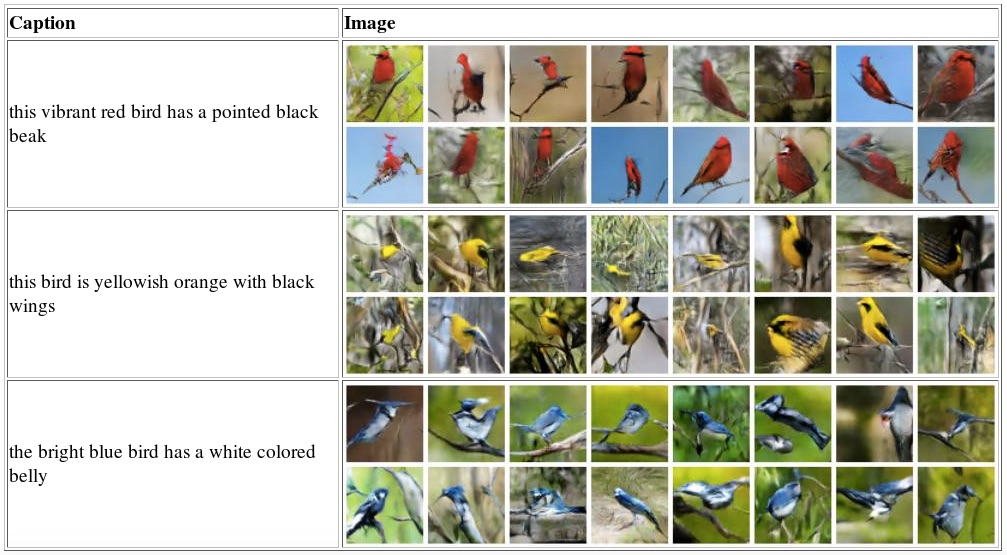
\includegraphics[width=\textwidth]{images/stackgan.jpg}
        \end{figure}
    \end{center}
    \footnote{Source: \url{https://github.com/reedscot/icml2016}}
\end{frame}

\begin{frame}
    \frametitle{Drawbacks of GANs}
    \begin{itemize}
        \item {GANs does not have an easily understood loss function.}
        \pause \item {It makes training GANs a lot harder.}
        \pause \item {A lot of trial and error is required to determine the network 
        structure and training protocol of GANs. This is the reason why GANs 
        have not been applied yet to more complex data like text or voices.}
    \end{itemize}
\end{frame}

\begin{frame}
    \begin{center}
        \LARGE{Thank You!}
    \end{center}
\end{frame}
\end{document}
